\documentclass[11pt]{article}
\usepackage[utf8]{inputenc}
\usepackage[margin=1in]{geometry}
\usepackage{setspace}
\usepackage[pdftex]{graphicx}
\DeclareGraphicsExtensions{.jpg}

\begin{document}

\title{Code and Analysis 5 Figures with Legends}
\author{Jonathan Lee and Danielle Covarrubias}
\maketitle

\iffalse
You can give your figures a label, then reference it in the text. When you include figures in your paper, you should always refer the reader to the figure and use it to clarify the text.

The conclusion statement for figure \ref{fig_sim} is this.

\begin{figure}[!h]
\centering
\includegraphics[width=2.5in]{agraph}
\caption{Here is where you put your legend for your figure.}
\label{fig_sim}
\end{figure}

The placement of figures can be difficult. Latex will decide where to
place the figure so it might appear in the same order as it is in the
tex document, or it might end up higher or lower on the page. It might
even be put at the end of the document if it is too big. You can try
to convince latex to put it here with [!h].

The conclusion statement for figure \ref{double_fig} is this.

\begin{figure}[!h]
  \centering
  \begin{tabular}[b]{c}
    \includegraphics[width=.3\linewidth]{subone} \\
    \small (a)
  \end{tabular} \qquad
  \begin{tabular}[b]{c}
    \includegraphics[width=.25\linewidth]{subtwo} \\
    \small (b)
  \end{tabular}
  \caption{Comparison of steady state results (a)~x method (b)~y method}
  \label{double_fig}
\end{figure}

--------------------------------- starting assignment----------------------------------
\fi

In these experiments, we measured the 3 following parameters against a range of input sizes for each problem:
% Table generated by Excel2LaTeX from sheet 'Sheet1'
% Table generated by Excel2LaTeX from sheet 'Sheet1'
\begin{table}[htbp]
  \centering
    \begin{tabular}{cl}
    1     & Node Count \\
    2     & Frontier Count \\
    3     & Depth \\
    \end{tabular}%
  \label{tab:addlabel}%
\end{table}%

By capturing the number of nodes expanded, we are able to measure the time complexity of each algorithm. In order to measure space complexity of each algorithm, we also kept track of the max frontier count in each experiment. Knowing the depth that the program reached until it ran out of time or memory is a good indicator of how far each algorithm can get based on the size of the input.

The parameters used for the simulated annealing experiments were as follows:\\~\\
\textbf{Parameter 1 (default)}\\
max\_time = 100 \ (arbitrary maximum time for any given task)\\
n = 20 \ (number of jobs)\\
p = 5 \ (number of people)\\~\\
\textbf{Parameter 2 (twice as many people as default)}\\
max\_time = 100 \ (arbitrary maximum time for any given task)\\
n = 20 \ (number of jobs)\\
p = 10 \ (number of people)\\~\\
\textbf{Parameter 3 (half as many jobs as default)}\\
max\_time = 100 \ (arbitrary maximum time for any given task)\\
n = 10 \ (number of jobs)\\
p = 5 \ (number of people)\\~\\

\pagebreak
The largest possible input size for both Queens and Towers was experimentally found to be:\\~\\
\textbf{N-Queens}\\
IDDFS Tree – 11 Queens (3.5 hours to compile)\\
BFS Tree – 8 Queens (stopped running after 1.5 hours)\\~\\
\textbf{Towers of Hanoi}\\
BFS Graph - 11 disks (timed out after 1 hour)\\
DFS Graph - 12 disks (timed out after 1 hour)\\
IDDFS Graph - 5 disks (timed out after 1 hour)


% Table generated by Excel2LaTeX from sheet 'Sheet1'
\begin{table}[!h]
  \centering
  \caption{NQueens - BFS Tree Search vs. IDDFS Tree Search}
    \begin{tabular}{|c|c|c|c|}
    \hline
          & \textbf{Max Depth} & \textbf{Node Count} & \textbf{Max frontier Count} \\
    \hline
        BFS Tree Problem Size &       &       &         \\
    \hline
     4 & 4     & 201   & 149 \\
    5 & 5     & 1,141 & 911 \\
    6 & 6     & 22,093 & 18,409 \\
     7 & 7     & 182,610 & 156,521 \\
    8 & 6     & 1,271,436 & 1,155,848 \\
    \hline
     IDDFS Tree Problem Size &       &       &         \\
     \hline
    4 & 4     & 97    & 7 \\
    5 & 5     & 363   & 11 \\
    6 & 6     & 2,475 & 16 \\
    7 & 7     & 14,225 & 22 \\
    8 & 8     & 117,344 & 29 \\
    11 & 11    & 109,761,332 & 56 \\
        \hline

    \end{tabular}%
  \label{nqueens}%
\\~\\
  \vspace*{5mm}
As shown in Table \ref{nqueens}, IDDFS tree search outperforms BFS tree search on every single problem size in terms of nodes generated and the maximum number of nodes in the frontier, highlighting its  superior runtime and memory use over the BFS tree algorithm.
\end{table}%



% Table generated by Excel2LaTeX from sheet 'Sheet1'
\begin{table}[htpb]
  \centering
  \caption{Simulated Annealing in Job Scheduling - Default: time = 100, jobs = 20, people = 5}
    \begin{tabular}{|c|c|c|c|c|}
    \hline
     & \textbf{Total iterations} & \textbf{Moves to better states} & \textbf{Moves to worse states} & \textbf{No moves} \\
       \hline
    Default &       &       &       &  \\
           \hline

    Trial 1 & 364,001 & 199,018 & 55,034 & 109,949 \\
    Trial 2 & 364,001 & 205,758 & 54,470 & 103,773 \\
    Trial 3 & 364,001 & 208,336 & 55,816 & 99,849 \\
    Trial 4 & 364,001 & 203,809 & 55,338 & 104,854 \\
    Trial 5 & 364,001 & 207,608 & 55,129 & 101,264 \\
    Average & 364,001 & 204,906 & 55,157 & 103,938 \\
        \hline
    people = 10 &       &       &       &  \\
           \hline

    Trial 1 & 364,001 & 220,800 & 43,134 & 100,067 \\
    Trial 2 & 364,001 & 222,877 & 43,830 & 97,294 \\
    Trial 3 & 364,001 & 219,769 & 43,966 & 100,266 \\
    Trial 4 & 364,001 & 226,104 & 42,036 & 95,861 \\
    Trial 5 & 364,001 & 227,113 & 42,555 & 94,333 \\
    Average & 364,001 & 223,333 & 43,104 & 97,564 \\
        \hline
    jobs = 10 &       &       &       &  \\
           \hline

    Trial 1 & 364,001 & 205,941 & 60,374 & 97,686 \\
    Trial 2 & 364,001 & 199,641 & 62,261 & 102,099 \\
    Trial 3 & 364,001 & 201,226 & 60,857 & 101,918 \\
    Trial 4 & 364,001 & 200,629 & 61,497 & 101,875 \\
    Trial 5 & 364,001 & 202,767 & 60,972 & 100,262 \\
    Average & 364,001 & 202,041 & 61,192 & 100,768 \\
    \hline
    \end{tabular}%
  \label{simulated_annealing}%
  \\~\\
  \vspace*{5mm}
  From the results of Table \ref{simulated_annealing}, doubling the number of people in job scheduling using simulated annealing, on average, results in a more efficient state whereas halving the number of jobs tends to yield a worse state when comparing them to the default parameters.
\end{table}%


% Table generated by Excel2LaTeX from sheet 'Sheet1'
\begin{table}[htpb]
  \centering
  \caption{Towers BFS-Graph}
    \begin{tabular}{|c|c|c|c|c|c|}
    \hline
    \# of disks & \textbf{3} & \textbf{6} & \textbf{8} & \textbf{10} & \textbf{11} \\
    \hline
    Total Node Count & 54    & 1932  & 18660 & 173052 & 514704 \\
    Max Frontier Count & 6     & 42    & 170   & 682   & 1024 \\
    Depth & 7     & 63    & 255   & 1023  & 2044 \\
    \hline
    \end{tabular}%
  \label{bfs_tower}%
  \\
  \vspace*{5mm}
  When BFS-graph search was used to find a solution for Towers, it can be seen in Table \ref{bfs_tower} that the program times out after 11 disks.
\end{table}%

% Table generated by Excel2LaTeX from sheet 'Sheet1'
\begin{table}[htpb]
  \centering
  \caption{Towers DFS-Graph}
    \begin{tabular}{|c|c|c|c|c|c|}
    \hline
    \# of disks & \textbf{3} & \textbf{5} & \textbf{9} & \textbf{11} & \textbf{12} \\
    \hline
    Total node count & 39    & 363   & 29523 & 265719 & 327855 \\
    Max frontier count & 8     & 63    & 4925  & 44292 & 54647 \\
    Depth & 13    & 121   & 9841  & 88573 & 109285 \\
    \hline
    \end{tabular}%
  \label{tower_dfs}%
  \\
  \vspace*{5mm}
  In Table \ref{tower_dfs}, DFS-graph search times out after 12 disks, which is a better time complexity improvement from BFS.
\end{table}%

% Table generated by Excel2LaTeX from sheet 'Sheet1'
\begin{table}[htpb]
  \centering
  \caption{Towers IDDFS-Graph}
    \begin{tabular}{|c|c|c|c|}
    \hline
    \# of disks & \textbf{3} & \textbf{4} & \textbf{5} \\
    \hline
    Total node count & 1495  & 12801757 & 350694110 \\
    Max frontier count & 14    & 30    & 36 \\
    Depth & 7     & 15    & 18 \\
    \hline
    \end{tabular}%
  \label{tower_iddfs}%
  \\~\\
  \vspace*{5mm}
  Solving Towers using ID-DFS graph search can be seen in Table \ref{tower_iddfs}, where the program timed out after 5 disks; the time complexity is significantly bigger compared to BFS and DFS.
\end{table}%

\begin{figure}[!h]
{\centering
\includegraphics[width=5in]{NodeCount.jpg}
\caption{Towers Experiments Total Node Count Results}
\label{tower_node}
}
\vspace*{5mm}
Looking at Figure \ref{tower_node}, IDDFS-graph exponentially expands more nodes compared to the linear trends of BFS-graph and DFS-graph, resulting in IDDFS-graph to have a much bigger time complexity than the other two algorithms.\\
\end{figure}



\begin{figure}[!h]
{\centering
\includegraphics[width=5in]{Frontier.jpg}
\caption{Towers Experiments Max Frontier Count Results}
\label{tower_frontier}
}
\vspace*{5mm}
According to Figure \ref{tower_frontier}, DFS-graph had the largest frontier count, which means it would essentially have a bigger space complexity than the other two; all 3 algorithms timed out before they ran out of memory.\\
\end{figure}



\begin{figure}[!h]
{\centering
\includegraphics[width=5in]{Depth.jpg}
\caption{Towers Experiments Depth Results}
\label{tower_depth}
}
\vspace*{5mm}
Based on Figure \ref{tower_depth}, DFS-graph search always reached the deepest nodes in the graph, which is where the solution can be found the quickest, hence why it performed the best. IDDFS timed out quickly because it would never reach the solutions at the depths of the graph.\\
\end{figure}


\begin{figure}[!h]
{\centering
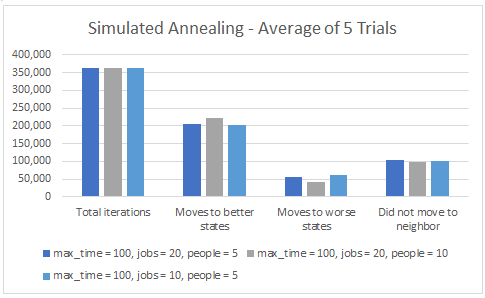
\includegraphics[width=5in]{sa.png}
\caption{Simulated Annealing Experiments Results}
\label{sa}
}
 \vspace*{5mm}
Figure \ref{sa} displays an improvement in returning a more optimal state when doubling the number of people and comparing the results to the default parameter with regards to job scheduling using simulated annealing.\\
\end{figure}

\begin{figure}[!h]
{\centering
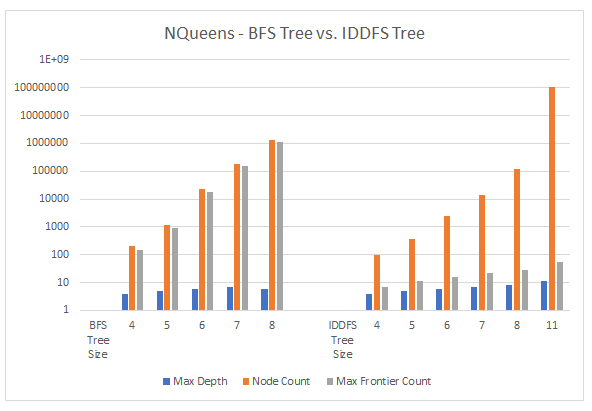
\includegraphics[width=5in]{nqueens.png}
\caption{NQueens Experiments Results}
\label{nqueens}
}
 \vspace*{5mm}
Figure \ref{nqueens} highlights the great difference between space and time complexity of IDDFS tree search and BFS tree search, respectively, as applied to the problem of NQueens.\\
\end{figure}



\end{document}
